% Options for packages loaded elsewhere
\PassOptionsToPackage{unicode}{hyperref}
\PassOptionsToPackage{hyphens}{url}
\PassOptionsToPackage{dvipsnames,svgnames,x11names}{xcolor}
\documentclass[
  10pt,
  fontset=fandol]{ctexart}
\usepackage{xcolor}
\usepackage[margin=16mm]{geometry}
\usepackage{amsmath,amssymb}
\setcounter{secnumdepth}{-\maxdimen} % remove section numbering
\usepackage{iftex}
\ifPDFTeX
  \usepackage[T1]{fontenc}
  \usepackage[utf8]{inputenc}
  \usepackage{textcomp} % provide euro and other symbols
\else % if luatex or xetex
  \usepackage{unicode-math} % this also loads fontspec
  \defaultfontfeatures{Scale=MatchLowercase}
  \defaultfontfeatures[\rmfamily]{Ligatures=TeX,Scale=1}
\fi
\usepackage{lmodern}
\ifPDFTeX\else
  % xetex/luatex font selection
\fi
% Use upquote if available, for straight quotes in verbatim environments
\IfFileExists{upquote.sty}{\usepackage{upquote}}{}
\IfFileExists{microtype.sty}{% use microtype if available
  \usepackage[]{microtype}
  \UseMicrotypeSet[protrusion]{basicmath} % disable protrusion for tt fonts
}{}
\makeatletter
\@ifundefined{KOMAClassName}{% if non-KOMA class
  \IfFileExists{parskip.sty}{%
    \usepackage{parskip}
  }{% else
    \setlength{\parindent}{0pt}
    \setlength{\parskip}{6pt plus 2pt minus 1pt}}
}{% if KOMA class
  \KOMAoptions{parskip=half}}
\makeatother
\usepackage{graphicx}
\makeatletter
\newsavebox\pandoc@box
\newcommand*\pandocbounded[1]{% scales image to fit in text height/width
  \sbox\pandoc@box{#1}%
  \Gscale@div\@tempa{\textheight}{\dimexpr\ht\pandoc@box+\dp\pandoc@box\relax}%
  \Gscale@div\@tempb{\linewidth}{\wd\pandoc@box}%
  \ifdim\@tempb\p@<\@tempa\p@\let\@tempa\@tempb\fi% select the smaller of both
  \ifdim\@tempa\p@<\p@\scalebox{\@tempa}{\usebox\pandoc@box}%
  \else\usebox{\pandoc@box}%
  \fi%
}
% Set default figure placement to htbp
\def\fps@figure{htbp}
\makeatother
\setlength{\emergencystretch}{3em} % prevent overfull lines
\providecommand{\tightlist}{%
  \setlength{\itemsep}{0pt}\setlength{\parskip}{0pt}}
\usepackage{amsmath,amssymb,mathtools,needspace}
\xeCJKDeclareCharClass{CJK}{"2032,"0400->"04FF,"2160->"216B,"2460->"2473,"25A0,"25C7,"25CB,"25CF}
\IfFontExistsTF{Arial Unicode MS}{\xeCJKsetup{AutoFallBack=true}\setCJKfallbackfamilyfont{\CJKrmdefault}{Arial Unicode MS}}{}
\setcounter{secnumdepth}{0}
\setlength{\emergencystretch}{2em}
\allowdisplaybreaks
\usepackage{bookmark}
\IfFileExists{xurl.sty}{\usepackage{xurl}}{} % add URL line breaks if available
\urlstyle{same}
\hypersetup{
  pdftitle={引言},
  colorlinks=true,
  linkcolor={Maroon},
  filecolor={Maroon},
  citecolor={Blue},
  urlcolor={Blue},
  pdfcreator={LaTeX via pandoc}}

\title{引言}
\author{}
\date{}

\begin{document}
\maketitle

\subsubsection{9.3.1 引言}\label{ux5f15ux8a00}

前面几节讨论的是求解矩阵最大（小）特征值及其对应特征向量的方法。若要求求出所有特征值及其特征向量，应该用什么方法呢？下面将讨论的以正交相似变换为基础的一类方法即是解决这类问题的方法。

首先，讨论对于一般实矩阵 \(A\in\mathbf R^{n\times n}\) 利用正交相似变换约化到什么程度的问题。由代数知识可知如下定理。

\textbf{定理 9.10} 设 \(A\in\mathbf R^{n\times n}\)，则存在一个正交阵 \(R\)，使

\[
R^{\mathrm T}AR=\begin{pmatrix}
T_{11}&T_{12}&\cdots&T_{1s}\\
&T_{22}&\cdots&T_{2s}\\
&&\ddots&\vdots\\
&&&T_{ss}
\end{pmatrix},
\]

其中对角块为一阶或二阶矩阵，每一个一阶对角块即为 \(A\) 的实特征值，每一个二阶对角块的两个特征值是 \(A\) 的一对共轭复特征值。

\textbf{定义 9.2} 一方阵 \(B\)，如果当 \(i>j+1\) 时有 \(b_{ij}=0\)，则称 \(B\) 为上 Hessenberg 阵，即

\[
B=\begin{pmatrix}
b_{11}&b_{12}&\cdots&b_{1n}\\
b_{21}&b_{22}&\cdots&b_{2n}\\
&\ddots&\ddots&\vdots\\
&&b_{n,n-1}&b_{nn}
\end{pmatrix}.
\]

本节讨论如下两个问题：

（1）用正交相似变换约化一般实矩阵为上 Hessenberg 阵；

（2）用正交相似变换约化对称阵为三对角阵。

这样，求原矩阵特征值问题，就转化为求上 Hessenberg 阵或对称三对角阵的特征值问题。

\textbf{定义 9.3} 设向量 \(w\) 满足 \(\|w\|_2=1\)，矩阵 \(H=I-2ww^{\mathrm T}\) 称为初等反射阵，记作 \(H(w)\)，即

\[
H(w)=\begin{pmatrix}
1-2w_1^2&-2w_1w_2&\cdots&-2w_1w_n\\
-2w_2w_1&1-2w_2^2&\ddots&\vdots\\
\vdots&\ddots&\ddots&-2w_{n-1}w_n\\
-2w_nw_1&\cdots&-2w_nw_{n-1}&1-2w_n^2
\end{pmatrix},
\]

\href{../../source-images/pdf-244.jpeg}{原页图像}

其中

\[
w=(w_1,w_2,\cdots,w_n)^{\mathrm T}.
\]

\textbf{定理 9.11} 初等反射阵 \(H\) 是对称阵（\(H^{\mathrm T}=H\)）、正交阵（\(H^{\mathrm T}H=I\)）和对合阵（\(H^2=I\)）。

\textbf{证明} 只证 \(H\) 的正交性，其他显然。

\[
H^{\mathrm T}H=H^2=(I-2ww^{\mathrm T})(I-2ww^{\mathrm T})=I-4ww^{\mathrm T}+4w(w^{\mathrm T}w)w^{\mathrm T}=I.
\]

设向量 \(u\ne0\)，则显然 \(H=I-2\dfrac{uu^{\mathrm T}}{\|u\|_2^2}\) 是一个初等反射阵。

下面考察初等反射阵的几何意义。考虑以 \(w\) 为法向量过原点 \(O\) 的超平面

\[
S:w^{\mathrm T}x=0.
\]

设任意向量 \(v\in\mathbf R^n\)，则 \(v=x+y\)，其中 \(x\in S,y\in S^{\perp}\)。于是

\[
Hx=(I-2ww^{\mathrm T})x=x-2ww^{\mathrm T}x=x.
\]

对于 \(y\in S^{\perp}\)，易知 \(Hy=-y\)，从而对于任意向量 \(v\in\mathbf R^n\)，总有

\[
Hv=x-y=v',
\]

其中 \(v'\) 为 \(v\) 关于平面 \(S\) 的镜面反射（见图 9.1）。

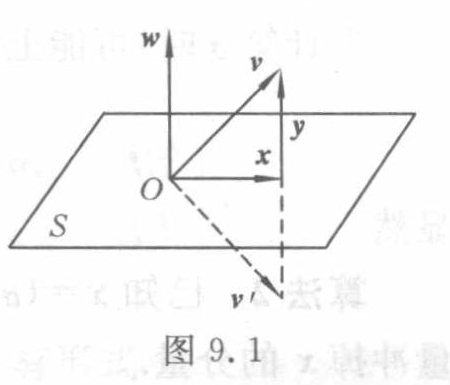
\includegraphics[width=0.85\linewidth,height=\textheight,keepaspectratio,alt={图 9.1，初等反射阵的几何意义，原图裁切}]{../assets/ch09a/fig-9-1.png}

图 9.1（原图裁切）。图中符号为 \(w,\allowbreak v,\allowbreak x,\allowbreak y,\allowbreak O,\allowbreak S,\allowbreak v'\)。超平面 \(S\) 经过原点 \(O\)，\(w\) 为法向量；\(v=x+y\) 分解为平面内分量 \(x\) 与垂直分量 \(y\)，\(v'\) 位于平面另一侧，表示镜面反射所得 \(x-y\)。原图用虚线连接 \(O\)、\(v'\) 端点及垂直分量方向。

初等反射阵在计算上的意义是它能用来约化矩阵，例如设向量 \(a\ne0\)，可选择一初等反射阵 \(H\) 使 \(H_a=\sigma e_1\)。这种约化矩阵的方法称为 Householder 方法。为此给出下面定理。

\textbf{定理 9.12} 设 \(x,y\) 为两个不相等的 \(n\) 维向量，\(\|x\|_2=\|y\|_2\)，则存在一个初等反射阵 \(H\)，使 \(Hx=y\)。

\textbf{证明} 令 \(w=\dfrac{x-y}{\|x-y\|_2}\)，则得到一个初等反射阵

\[
H=I-2ww^{\mathrm T}=I-2\frac{(x-y)}{\|x-y\|_2^2}(x^{\mathrm T}-y^{\mathrm T}),
\]

而且

\[
Hx=x-2\frac{x-y}{\|x-y\|_2^2}(x^{\mathrm T}-y^{\mathrm T})x=x-2\frac{(x-y)(x^{\mathrm T}x-y^{\mathrm T}x)}{\|x-y\|_2^2},
\]

因为

\[
\|x-y\|_2^2=(x-y)^{\mathrm T}(x-y)=2(x^{\mathrm T}x-y^{\mathrm T}x),
\]

所以

\[
Hx=x-(x-y)=y.
\]

易知，\(w=\dfrac{x-y}{\|x-y\|_2}\) 是使 \(Hx=y\) 成立的唯一长度等于 1 的向量（不计符号）。

\textbf{推论} 设向量 \(x\in\mathbf R^n\ (x\ne0)\)，\(\sigma=\pm\|x\|_2\)，且 \(x\ne-\sigma e_1\)，则存在一个初等反射阵

\[
H=I-2\frac{uu^{\mathrm T}}{\|u\|_2^2}\equiv I-\rho^{-1}uu^{\mathrm T},
\]

使 \(Hx=-\sigma e_1\)，其中 \(u=x+\sigma e_1\)，\(\rho=\|u\|_2^2/2\)。

设

\[
x=(\alpha_1,\alpha_2,\cdots,\alpha_n)^{\mathrm T}\ne0,\quad u=(u_1,u_2,\cdots,u_n)^{\mathrm T},
\]

\begin{quote}
\textbf{校注（agent 补充，ch09a-E008）} 在``可选择一初等反射阵 \(H\) 使''后，原图把 \(a\) 印在 \(H\) 的下标位置，故照录为 \(H_a=\sigma e_1\)。依本段语义及随后定理的矩阵作用，应为乘积 \(Ha=\sigma e_1\)；疑为原书排版错误。见\href{../assets/ch09a/review-p244-Ha.png}{放大原式}。
\end{quote}

\href{../../source-images/pdf-245.jpeg}{原页图像}

则

\[
u=(\alpha_1+\sigma,\alpha_2,\cdots,\alpha_n)^{\mathrm T},
\]

\[
\rho=\frac12\|u\|_2^2=\frac12\left[(\alpha_1+\sigma)^2+\alpha_2^2+\cdots+\alpha_n^2\right]=\sigma(\sigma+\alpha_1).
\]

如果 \(\sigma\) 和 \(\alpha_1\) 异号，那么计算 \(\alpha_1+\sigma\) 时有效数字可能损失，取 \(\sigma\) 和 \(\alpha_1\) 有相同的符号，即取

\[
\sigma=\operatorname{sgn}(\alpha_1)\|x\|_2.
\]

\textbf{算法 1} 已知向量 \(x=(\alpha_1,\alpha_2,\cdots,\alpha_n)^{\mathrm T}\ne0\)，本算法算出 \(\sigma,\rho\) 及 \(u\)，使 \((I-\rho^{-1}uu^{\mathrm T})x=-\sigma e_1\)，\(u\) 的分量冲掉 \(x\) 的分量。

\textbf{步 1} 计算 \(\sigma=\operatorname{sgn}(\alpha_1)\left(\displaystyle\sum_{i=1}^n\alpha_i^2\right)^{\frac12}\)。

\textbf{步 2} \(\alpha_1\to u_1=\alpha_1+\sigma\)。

\textbf{步 3} \(\rho=\sigma u_1\)。

在计算 \(\sigma\) 时，可能上溢或下溢。为了避免溢出，将 \(x\) 规范化

\[
\eta=\max_i|\alpha_i|,\quad x'=\frac{x}{\eta},
\]

显然

\[
\sigma'=\sigma/\eta,\quad H'=H.
\]

\textbf{算法 2} 已知 \(x=(\alpha_1,\alpha_2,\cdots,\alpha_n)^{\mathrm T}\ne0\)，本算法算出 \(H\) 及 \(\sigma\) 使 \(Hx=-\sigma e_1\)，\(u\) 的分量冲掉 \(x\) 的分量。

\textbf{步 1} \(\eta=\max_i|\alpha_i|\)。

\textbf{步 2} \(\alpha_i\leftarrow u_i=\dfrac{\alpha_i}{\eta}\quad(i=1,2,\cdots,n)\)。

\textbf{步 3} \(\sigma=\operatorname{sgn}(u_1)\left(\displaystyle\sum_{i=1}^nu_i^2\right)^{\frac12}\)。

\textbf{步 4} \(u_1\leftarrow u_1+\sigma\)。

\textbf{步 5} \(\rho=\sigma u_1\)。

\textbf{步 6} \(\sigma\leftarrow\eta\sigma\)。

关于 \(HA\) 的计算，设 \(A=(a_1,a_2,\cdots,a_n)\)，其中 \(a_i\) 为 \(A\) 的第 \(i\) 列向量，则

\[
HA=(Ha_1,Ha_2,\cdots,Ha_n),
\]

因此计算 \(HA\) 就是要计算

\[
Ha_i=(I-\rho^{-1}uu^{\mathrm T})a_i=a_i-(\rho^{-1}u^{\mathrm T}a_i)u\quad(i=1,2,\cdots,n).
\]

于是计算 \(Ha_i\) 只需要计算两向量的数量积和两向量的加法即可，且计算 \(HA\) 共需要 \(2n^2\) 次乘法运算。

\subsection{本节覆盖原页的校注记录}\label{ux672cux8282ux8986ux76d6ux539fux9875ux7684ux6821ux6ce8ux8bb0ux5f55}

下列记录按原页关联，含同页相邻小节的校注；计算时同时读取上文校注和完整原页。

\begin{itemize}
\tightlist
\item
  \texttt{ch09a-E008}：原书 PDF 页 244
\end{itemize}

\end{document}
